\chapter{Einleitung}
\label{sec:einleitung} 



Die Computer Vision gehört zum Fachbereich der Computer Science und beinhaltet die Entwicklung von künstlichen Intelligenzen, allen voran dem Versuch Computern ein visuelles Verständnis ihrer Umgebung zu geben. Computer Vision behandelt den umgekehrten Weg des Bildes aus der Realität in den Rechner\cite{ComputerVision}. Die Fähigkeit die gesehenen Bilder zu verarbeiten und zu interpretieren erlaubt es dem Menschen ein Verständnis über die ihn umgebenen Welt zu erlangen. Computer, welche die Fähigkeit besitzen die Welt um sich herum wie das menschliche Auge zu betrachtet und aus diesen entstehenden Bildern Informationen zu extrahieren, wären dem zu folge auch in der Lage Entscheidungen auf Grund von visuellen Eindrücken zu fällen und entsprechend zu handeln. Ein derartiges Verhalten lässt sich in drei Schritte unterteilen. Die Bildaufnahme und Speicherung, die Bildverarbeitung und die Bildanalyse\cite{ComputerVision}. Als erstes wird die Umgebung in digitale, für der Computer verständliche, Bilder umgewandelt werden. Dies erfolgt mit Hilfe von Kameras, Sensoren oder Lasern. 
 Die Bildverarbeitung und die Bildanalys lassen sich unterteilen in die Detektion elementarer Merkmale wie Kanten, gerade Linien und Eckpunkte, Segmentierung, die Analyse elementarer Formen und die Identifikation von Objekten\cite{CamerModels.}.Für die Identifikation von Objekten, werden die zuvor berechneten speziellen Punkte aus den verschiedenen Bildern analysierte, um die 3D Strukturen der Objekte zu erhalten. 
% 
% mit Hilfe von Detektionsalgorithmen werden markante Punkte auf den aufgenommen Bilder herausgefiltert, dazu gehören beispielsweise die Kanten und Ecken-Erkennung, die Segmentierung von Bildern in einzelne sich nicht überlappende Teilbereiche und anschließende Klassifizierung sowie Merkmals Erkennungen.  
% 
% Der dritte Schritt ist dann eine Zusammenführung der ersten beide Schritte. Danach können aus den Bilddaten und den Merkmalen, welche durch den Bildverarbeitung entstanden sind, Informationen über die Umgebung berechnet werden \cite{ComputerVision}. 
%  Dazu gehören unter anderem das rekonstruieren des 3D-Raumes oder die Objekterkennung von Objekte im Raum, sowie auch deren Bewegungsverfolgung, falls diese nicht statisch sind. 
Beispiele für auf Computer Vision basierende Applikationen sind im Bereich des Autonomen Fahrens, Motion-Capturing-Anlagen, Bewegungserkennungen oder Service Robotern zu finden. Mit dem Entwickeln von Algorithmen für Computer Vision Applikationen, sieht man sich mit immer wieder mit komplizierten Aufgaben und Herausforderungen konfrontiert. Bei der Aufnahme von Bildern, kann es immer wieder zu unvorhersehbaren Bildfehlern wie beispielsweise Rauschen oder Verzerrungen durch die Kameralinse kommen, was auch nicht oft zum Verlust von Referenzdaten führt. In den Ergebnisse, des in dieser Arbeit verfassten Algorithmus für die Rekonstruktion einer stereoskopisch aufgenommenen Szene, sind Auswirkungen eben solcher Fehler zu erkennen. Im Kapitel \nameref{sec:real} wird aufgeführt, wie mit solchen Fehlern umgegangen werden kann.
%Des Weiteren muss mit limitierten Ressourcen wie Speicher oder Rechenleistung geschickt umgegangen werden, gerade im Bereich der Echt-Zeit-Verarbeitungen von Daten, wie sie im Motion-Capturing oder im autonomen Fahren verlangt werden. 
Computer Vision kommt immer dann zum Einsatz, sobald Informationen aus Bildern gewonnen werden sollen. Dabei kann man unterscheiden unter der Informationsgewinnung aus einzel Bildern oder bewegt Bildern, genauso wie single-view, two-view oder multiple-view Aufnahmen. Single-View beschreibt die Bildverarbeitung anhand der Aufnahmen einer Kamera, two-view befasst sich mit Stereoskopischen Aufnahmen und involviert zwei Kameras und multiple-view ist die Zusammenfassung von mehr als zwei Kameras, wie sie beispielsweise im Motion-Capturing verwendet werden\cite{HZ}. %
%Um eine dreidimensionale Interpretation von Objekten und deren Orientierung im Raum, basierend auf Bilddaten von Kameras, zu bekommen, muss in irgendeiner Form bestimmte Parameter des verwendeten Kameramodells bekannt sein oder herausgefiltert werden. 
Zur Analyse verschiedener Bilder ist es essentiell die verschiedenen Kameraparameter, wie Position und Auflösung, zu kennen. Diese können zuvor bestimmt werden, oder aus den Bildern mit Hilfe spezieller Modelle abgeleitet werden. Die Position und Rotation einer Kamera im Raum werden als die extrinsischen Kameraparameter bezeichnet und können durch eine $3\times4$-Matrix beschrieben werden. Die Parameter wie die Auflösung oder Brennweiten, werden als die intrinsischen Kameraparameter bezeichnet und können in einer $3 \times 3$-Matrix, die sogenannte Kameramatrix, ausgedrückt werden werden. Sind die Parameter nicht bekannt, so können sie durch die aus Bilddaten gewonnenen Informationen geschätzt werden. Das Verfahren wird als Kamerakalibrierung bezeichnet\cite{HZ,Ferid,Elements,ZZGXr}.

%Dieser Vorgang wird als Kamerakalibrierung bezeichnet und beschreibt die Gewinnung von extrinsischen und intrinsischen Kameraparametern.
% Als extrinsische oder auch äußeren Kameraparameter wir die Orientierung der Kamera im Raum beschrieben, diese wird in einer 3X4-Matrix ausgedrückt, welche sowohl die Rotation der Kamera also auch deren Translation umfässt. Die intrinsischen Kameraparameter oder auch inneren Kameraparameter werden in der sogenannten Kameramatrix zusammengefasst, welche je nach benutzten Kameramodell sich unterscheidet.
Die extrinsischen und intrinsischen Matrizen bilden zusammen die sogenannte Projektionsmatrix $P$, welche die komplette Transformation eines Dreidimensionalen Punktes $M$ im Raum in einen Zweidimensionalen Bildpunkt $m$ beschreibt mit $m = PM$. Im Kapitel \nameref{sec:CameraModels} wird das hier verwendete Kameramodell der Lockkamera und die extrinsischen und intrinsischen Kameraparameter und ihre jeweiligen Matrizen noch genauer vorgestellt. Sind die Kameraparameter bekannt, kann eine Szenerekonstruktion erfolgen. Die Szenenrekonstruktion beschreibt den Vorgang, in welchem Anhand von Bildpunkten und den bekannten Kameraparameter die Dreidimensionale Szene der Bilder rekonstruiert wird. Das Ziel dieser Masterarbeit ist es zum einen, mit Hilfe einer Stereoaufnahme einer Szene, eine Kamerakalibrierung und anschließend eine Szenenrekonstruktion durchzuführen. Die eigens implementierte Kamerakalibrierung befasst sich ausschließlich mit der Schätzung der extrinsischen Kameraparameter, für die intrinsischen wird auf ein bereits vorhandenes externes Programm zurückgegriffen. Danach erfolgt die Szenenrekonstruktion. Der eigens entwickelte Ansatz wird in zwei Schritten in dieser Arbeit vorgestellt. Im erste Schritt wird ein sogenanntes Minimalbeispiel aufgebaut. Das Minimlabeispiel beinhaltet eine synthetisch im Programm aufgebaute 3D-Szene. Die 3D-Szene wird dann in zwei voneinander unterschiedlich positionierten simulierten Kameras projiziert, so dass pro Kamera ein 2D-Bild des 2D-Objektes existiert. Anhand dieser 2D-Bilddaten soll dann eine Kalibrierung der extrinsischen Kameraparameter und anschließend eine Rekonstruktion der 3D-Szene erfolgen. Vorteil an diesem Minimalbeispiel ist, dass das Ergebnis der Rekonstruktion leicht abgeglichen werden kann und somit die Funktionalität des implementierten Algorithmus an einem reinen nicht verfälschten Fall getestet werden kann. Des Weiteren können Fehler welche im späteren Beispiel mit realen Bilddaten auftreten, in diesem synthetischen Aufbau rekonstruiert und somit mögliche Lösungen für diese gefunden werden. Abbildung \ref{fig:AbbildungenMinimal} zeigt noch einmal Schematisch den Arbeitsprozess des Minimalbeispiels. Die einzelnen Schritte in dieser Abbildung werden im Kapitel \nameref{sec:minimal} genauer erläutert. 


\begin{minipage}{\linewidth}
	\centering
	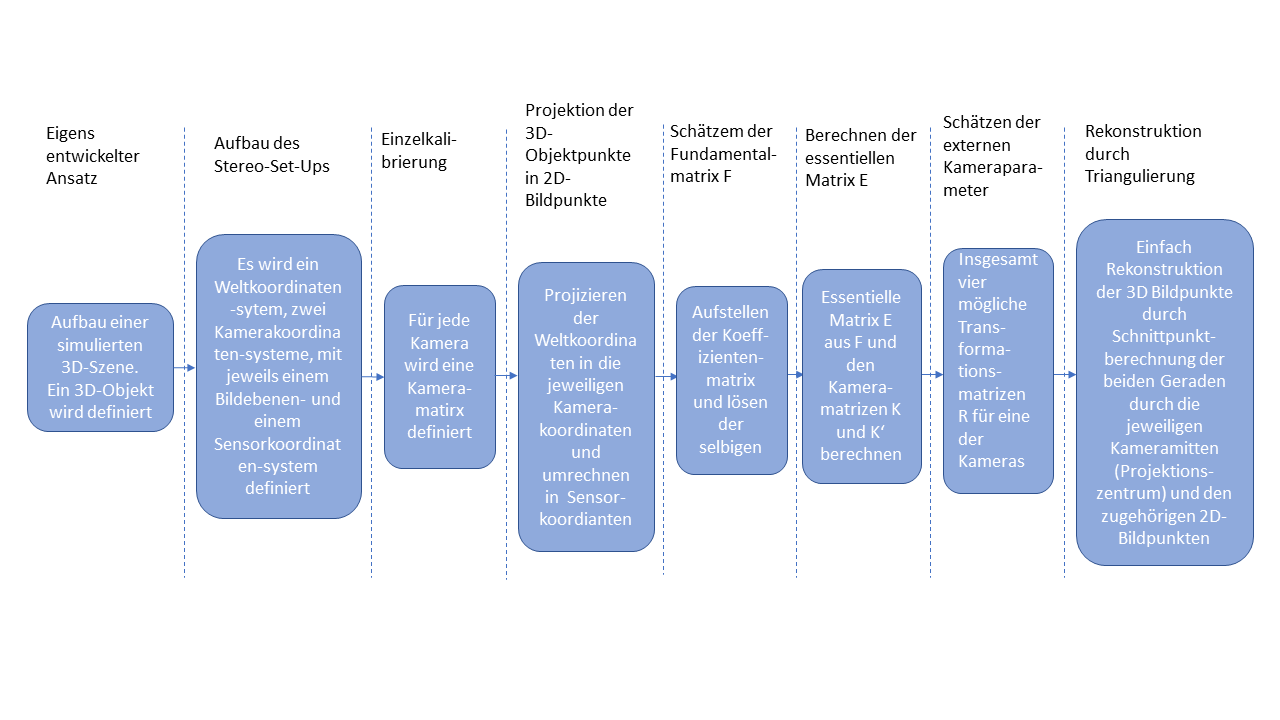
\includegraphics[width=1.\linewidth]{images/ArbeitsProzessMinimal.png}
	\captionof{figure}{Arbeitsprozesse der Stereoanalyse bei Verwendung von eigens erstellten synthetischen Bilddaten}
	\label{fig:ArbeitsProzessMinimal}
\end{minipage}\\ \\

Das Minimalbeispiel soll dabei einmal mit Kameras gleicher Auflösung und einmal mit Kameras unterschiedlicher Auflösung durchgerechnet werden. Eine Frage, die ebenfalls im Zuge der Arbeit beantwortet werden soll, ist welche Auswirkungen zwei Kameras mit unterschiedlichen Auflösungen auf den Prozess der Kamerakalibrierung und der Szenerekonstruktion haben. Die Stereokalibrierungs Applikation, welche von \textit{MatLab} bereitgestellt wird, ist nicht in der Lage eine Stereokalibrierung und Szenenrekonstruktion von zwei Bilder unterschiedlicher Auflösung zu machen. Im zuge dessen, wurde die Vorgehensweise der Applikation genauer betrachtet und den Auslöser dieses Problems gesucht. Der Arbeitsprozess, welcher in \textit{Matlab} für die Kamerakalibrierung und der anschließenden Szenerekonstruktion verfolgt wurde ist in Abbildung \ref{fig:ArbeitsProzessRealUnkalibriert} zu sehen. Der Grund warum die Stereoanalyse bei unterschiedlichen Kameraauflösungen in \textit{MatLab} nicht funktioniert wurde im Schritt der Rektifizierung ausgemacht. Im Kapitel \nameref{sec:rectification} wird nochmal explizit auf das Problem eingegangen und ein möglicher anderer Ansatz Aufgezeigt, welcher das Problem beheben könnte.

\begin{minipage}{\linewidth}
	\centering
	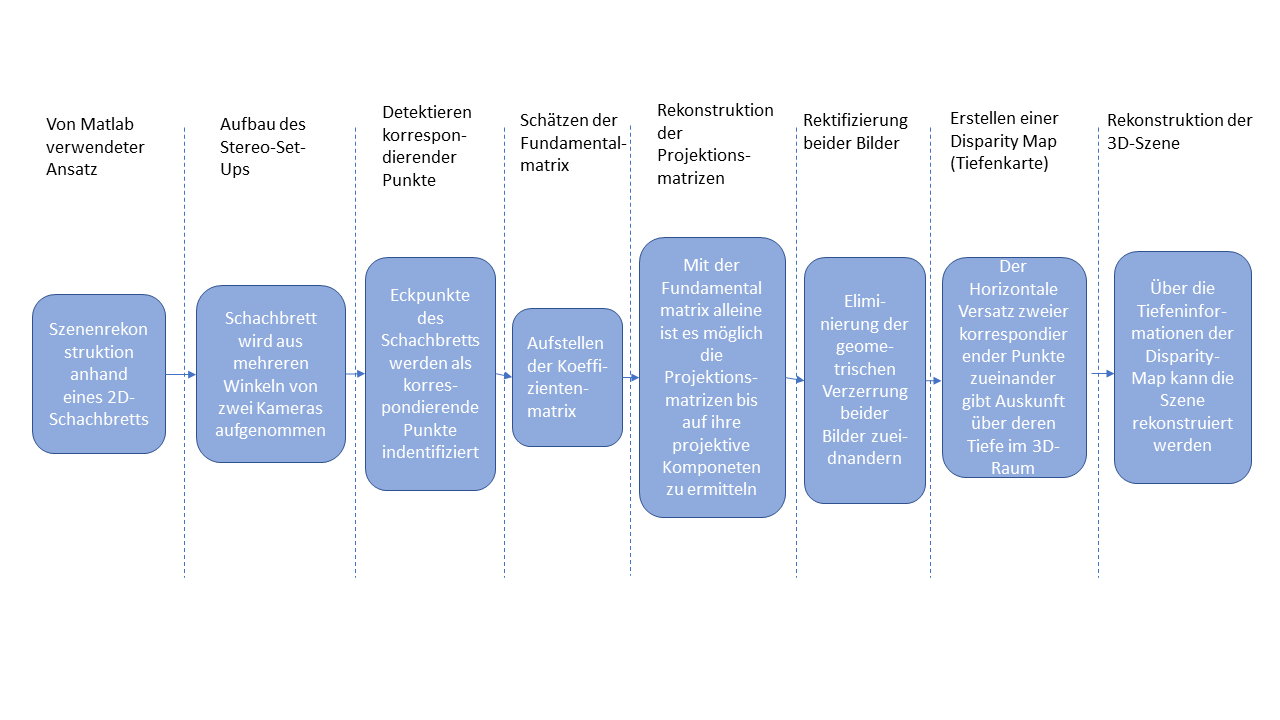
\includegraphics[width=1.\linewidth]{images/ArbeitsProzessRealunkalibriert.png}
	\captionof{figure}{Arbeitsprozesse der Stereoanalyse bei Verwendung von realen Bilddaten in einem unkalibrierten Fall}
	\label{fig:ArbeitsProzessRealUnkalibriert}
\end{minipage}\\ \\

Im zweiten großen Teil der Arbeit, soll der im Minimalbeispiel aufgebaute Algorithmus in einer realen Umgebung getestet werden. Es wird also ein Stereosystem mit zwei Kameras im Labor aufgebaut. Die intrinsischen Kameraparameter werden zuvor mit Hilfe eines externen Programms ermittelt. Danach nehmen die Kameras gleichzeitig einen realen Szenenaufbau aus zwei unterschiedlichen Positionen und Winkeln auf. Ab hier setzt der Algorithmus ein, welcher auch für das Minimalbeispiel genutzt wurde. Zuerst wird eine Kalibrierung der extrinsischen Kameraparameter durchgeführt und anschließend die Szene rekonstruiert. Im Kapitel \nameref{sec:real} wird des Weiteren noch drauf eingegangen, wie mit den genannten Bildfehlern, welche in Realaufnahmen entstehen können umgegangen wird, um die Auswirkungen dieser Fehler auf die Resultate so gering wie möglich zu halten. In Abbildung \ref{fig:ArbeitsProzessReal} ist der Arbeitsprozess für das Realbeispiel zu sehen. 

\begin{minipage}{\linewidth}
	\centering
	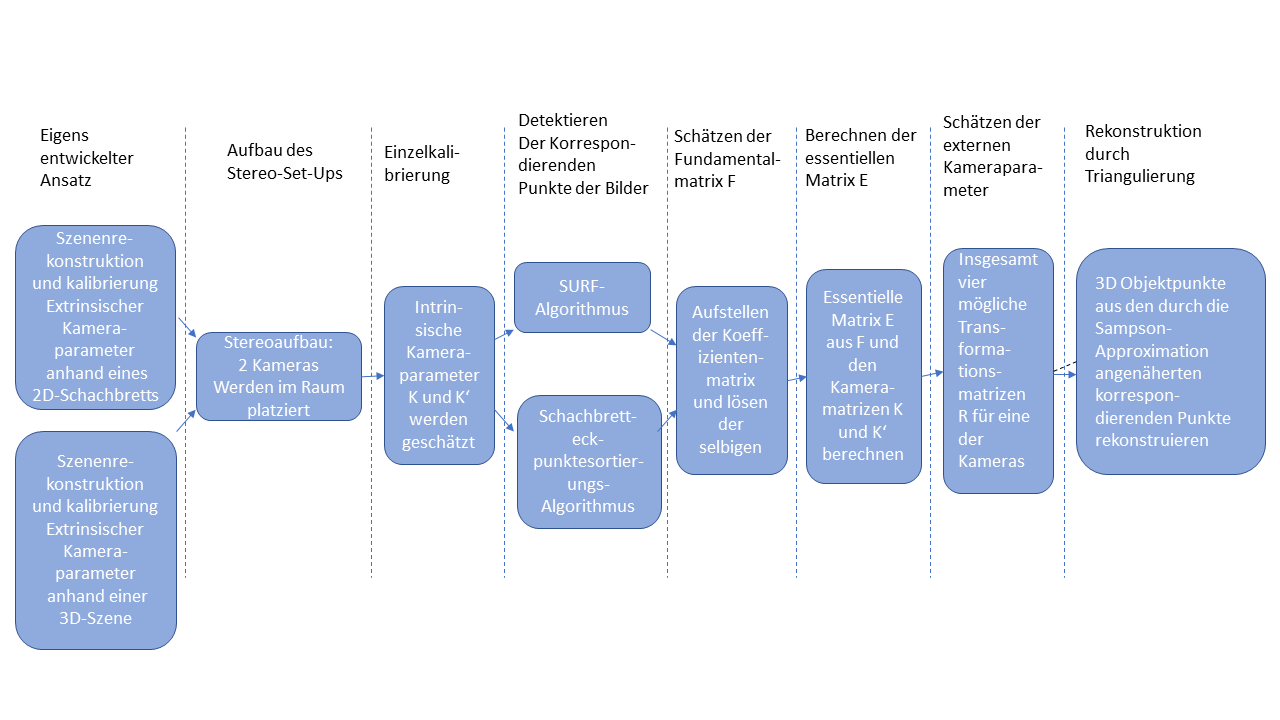
\includegraphics[width=1.\linewidth]{images/ArbeitsProzessReal.png}
	\captionof{figure}{Arbeitsprozesse der Stereoanalyse bei Verwendung von realen Bilddaten in einem kalibrierten Fall}
	\label{fig:ArbeitsProzessReal}
\end{minipage}\\ \\

Auch im Realbeispiel wird geprüft, ob unterschiedlicher Kameraauflösungen sich auf die Szenerekonstruktion auswirken und mit den Ergebnissen aus dem Minimalbeispiel verglichen.

% Diese nehmen jeweils die selbe Szene aus zwei unterschiedlichen Positionen und Winkeln auf. 
%
%Im Zuge dieser Masterarbeit, soll Anhand einer Stereoskopischen Aufnahme eine Kamerakalibrierung durchgeführt werden, um anschließend eine Szenerekonstruktion der Aufnahmen zu ermöglichen. Hierzu werden zwei Ansätze genauer betrachtet. Zum einen wird eine Komplette Rekonstruktion einer Szene mit einem kalibrierten Fall durch prozessiert. Kalibrierter Fall bedeutet in diesem Sinne, dass die intrinsischen Kameraparameter bekannt sind und mit Hilfe der sogenannten essentiellen Matrix die extrinsischen ermittelt werden sollen. Der zweite Ansatz bezieht sich auf den unkalibrierten Fall, in welchem keine Informationen über extrinsische und intrinsische Parameter vorliegen. Die Frage die im Zuge dieser zwei Ansätze beantwortet werden soll, ist welche Auswirkungen zwei Kameras mit unterschiedlichen Auflösungen auf den Prozess der Kamerakalibrierung und der Szenerekonstruktion haben.(noch weiter ausbauen...).

%Der im Verlauf dieser Arbeit entstandene Algorithmus führt eine Szenenrekonstruktion anhand des kalibrierten Beispiels aus, der unkalibrierte Fall ist nicht implementiert, jedoch ist dessen Vorgehen durch Die Stereokalibrierungs Applikation von \textit{MatLab}\cite{MatlabStereoApp} bekannt. Der implementierte Algorithmus wurde anhand einer synthetisch aufgebauten Szene theoretisch getestet und anschließend auf eine reale Stereoaufnahme angewandt. Die einzelnen Schritte des Algorithmus und woran sie sich unterscheiden sind in den Abbildungen \ref{fig:ArbeitsProzessMinimal} und \ref{fig:ArbeitsProzessReal} aufgezeigt. Im Verlauf dieser Arbeit werden die Hintergründe der einzelnen Schritte genauer beleuchtet.


%\begin{minipage}{\linewidth}
%	\centering
%	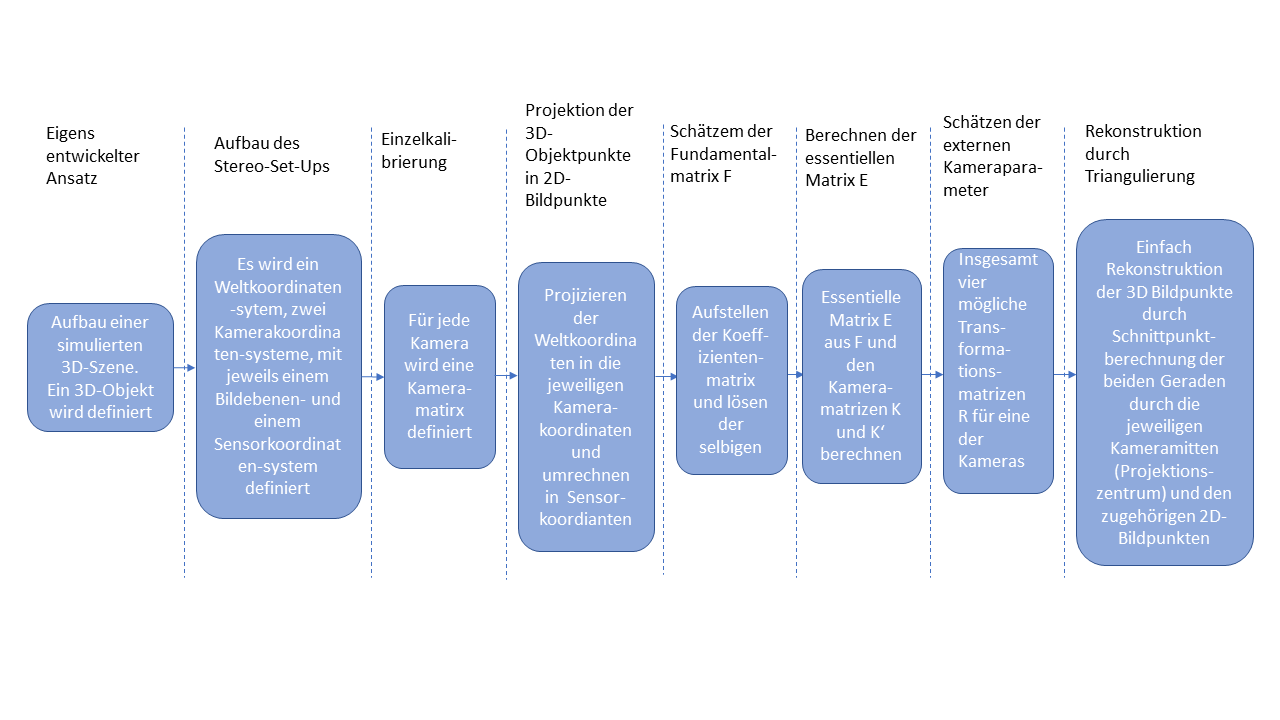
\includegraphics[width=1.\linewidth]{images/ArbeitsProzessMinimal.png}
%	\captionof{figure}{Arbeitsprozesse der Stereoanalyse bei Verwendung von eigens erstellten synthetischen Bilddaten}
%	\label{fig:ArbeitsProzessMinimal}
%\end{minipage}\\ \\
%
%
%\begin{minipage}{\linewidth}
%	\centering
%	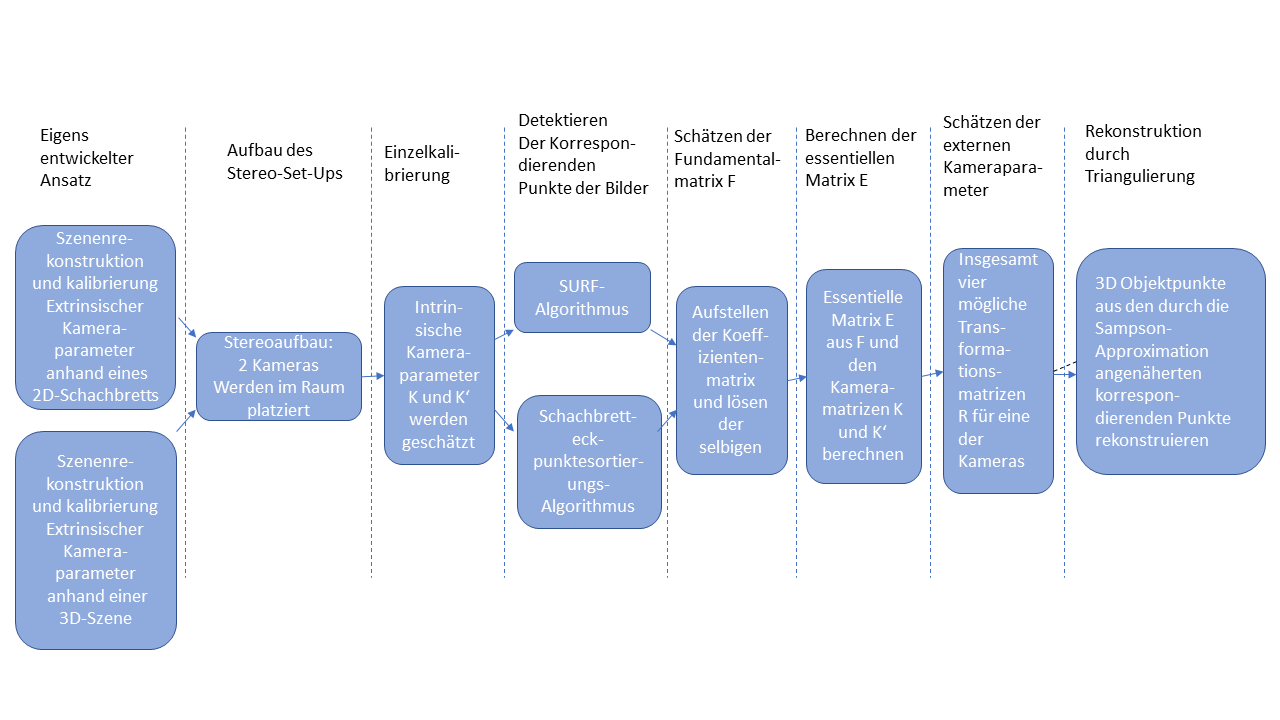
\includegraphics[width=1.\linewidth]{images/ArbeitsProzessReal.png}
%	\captionof{figure}{Arbeitsprozesse der Stereoanalyse bei Verwendung von realen Bilddaten in einem kalibrierten Fall}
%	\label{fig:ArbeitsProzessReal}
%\end{minipage}\\ \\
%
%
%Ein sehr wichtiger Aspekt dieses Ansatzes gerade im Bezug dann auch auf die Frage der Auswirkung von unterschiedlichen Kameraauflösungen auf die Szenerekonstruktion, ist die Epipolargeometrie. Sie beschreibt allem voran die zusammenhängende Geometrie zwischen den Bildpunkten zweier Bilder zueinander und deren geometrischen Zusammenhang zum 3D-Objektpunkt, was bei der Rekonstruktion der Szene besonders wichtig ist.\\

%
%\begin{minipage}{\linewidth}
%	\centering
%	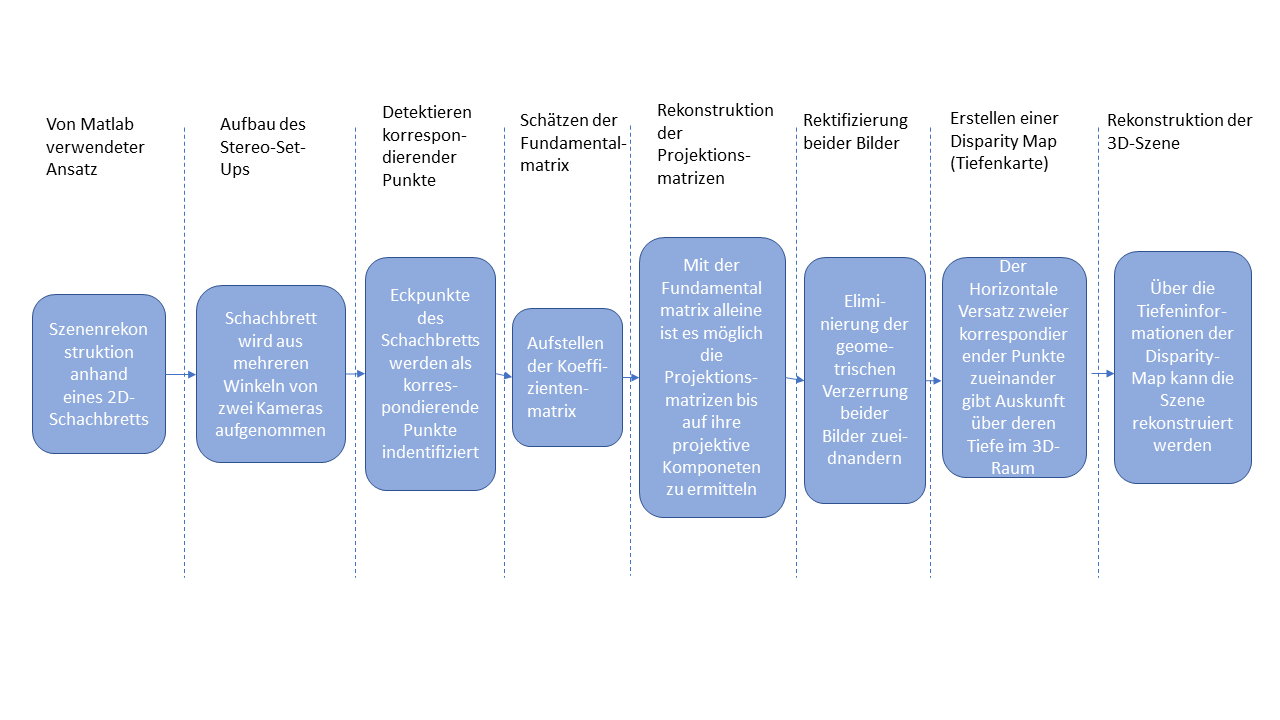
\includegraphics[width=1.\linewidth]{images/ArbeitsProzessRealunkalibriert.png}
%	\captionof{figure}{Arbeitsprozesse der Stereoanalyse bei Verwendung von realen Bilddaten in einem unkalibrierten Fall}
%	\label{fig:ArbeitsProzessRealUnkalibriert}
%\end{minipage}\\ \\
%
%
%In Abbildung \ref{fig:ArbeitsProzessRealUnkalibriert} ist der Arbeitsprozess des unkalibrierten Falles aufgezeigt, so wie er beispielsweise in \textit{Matlab} implementiert ist. Der elementare Schritt mit dem sich beschäftigt wird ist die Rektifizierung der Bilder. Im Schritt der Rektifizierung wird die sogenannte geometrische Verzerrung zweier Bilder eliminiert, was genau das Bedeutet wird im Kapitel \nameref{sec:rectification} beschrieben. Die Rektifizierung beinhaltet vorallem mathematische Operationen auf den 2D-Bildebenen der aufgenommenen 2D-Bilder, weshalb im Zuge dessen die Funktion und Herleitung von Homographien im Kapitel \nameref{sec:homographien} aufgezeigt werden. Der Grund warum die Rektifizierung in den Vordergrund gerückt wird, ist, das es Beispielswesise genau in diesem Schritt in \textit{Matlab} zu einem Problem kommt, wenn mit Kameras unterschiedlicher Auflösung gearbeitet wird. Die Herkunft des Problems wird im Verlauf der Arbeit geklärt und ein Ansatz für Minimierung dessen, wenn man den unkalibrierten Fall verfolgen möchte, wird aufgezeigt. Zu finden ist dies im Kapitel \nameref{sec:rectification}.Die Kapitel sind wie folgt gegliedert. 


Die Kapitel 1 bis 5 umfassen die theoretischen Mathematischen Hintergründe, welche für das Verständnis der implementierten Kalibrierungs- und Rekonstruktionsalgorithmen vorhanden sein müssen. Kapitel 6 beinhaltet die einzelnen Schritte des in Abbildung \ref{fig:ArbeitsProzessMinimal} aufgezeigten Kalibrierungs- und Rekonstruktionsalgorithmus des Minimalbeispiels. Mit diesem Kapitel werden die zuvor beschriebenen mathematischen Werkzeuge zusammengefasst und in Bezug der Stereoskopischen Szenenrekonstruktion angewandt. Der Grund der implentierung dieses Minimalbeispiels war unter anderem der, dass somit Fehler, welche im Realbeispiel aufgetreten sind rekonstruiert und eine mögliche Lösung dieser ermittelt werden konnte. Kapitel 7 geht auf die Problematik der unterschiedlichen Kamerauflösungen im Bezug auf die im Minimalbeispiel konstruierten Szene ein und führt auch noch auf, wie genau Auflösungen zustande kommen. Kapitel 8 und 9 transferieren dann den im Minimalbeispiel implementierten Algorithmus auf ein reales Beispiel mit einer echten Stereoskopischen Aufnahme. Die einzelnen Schritte aus Abbildung \ref{fig:ArbeitsProzessReal} werden hier ausführlichst besprochen. Das letzte Kapitel, Kapitel 10, bezieht sich auf einen Algorithmus welcher im Zuge des Realbeispiels enstanden ist. In Abbildung \ref{fig:ArbeitsProzessReal} ist im Ansatz der Punkt Kalibrierung anhand eines 2D-Schachbretts aufgeführt. Der in Kapitel 10 beschriebene Algorithmus, kann die zuvor detektierten Punkte eines Schachbretts in eine Gitterstruktur sortieren, selbst wenn es zu starken Bildfehlern wie Verzeichnugen kommt und das Schachbrett auf Grund seiner Lage auch noch projektiv verzerrt ist. Als Gitterstruktur sortiert bedeutet, dass die Punkte später wissen in welcher Zeile beziehungsweise Spalte sie sich im Gitternetz befinden und welches ihre Nachbarn sind. 

